
\section{Alfadian Owen}



 
 
\subsection{Sejarah python}


\qquad Bahasa pemrograman Python adalah bahasa yang dibuat oleh seorang keturunan Belanda yaitu Guido van Rossum. Awalnya, pembuatan bahasa pemrograman ini adalah untuk membuat skrip bahasa tingkat tinggi pada sebuah sistem operasi yang terdistribusi Amoeba. Python telah digunakan oleh beberapa pengembang dan bahkan digunakan oleh beberapa perusahaan untuk pembuatan perangkat lunak komersial.


\subsection{Instalasi Anaconda}
\begin{enumerate}
\item Download Terlebih dahulu aplikasi anaconda yang ada di https://www.anaconda.com/distribution/ 
\item Setelah download anda selesai, buka file yang anda download tadi
\item Klik next
\begin{figure}[H]
\centering
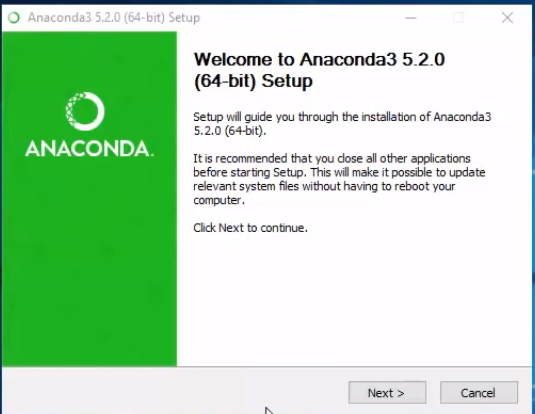
\includegraphics[width=6cm,height=6cm]{figures/gambar1.png}
\caption{Klik Next}
\label{akhir}
\end{figure}
\item Klik I Agree
\begin{figure}[H]
\centering
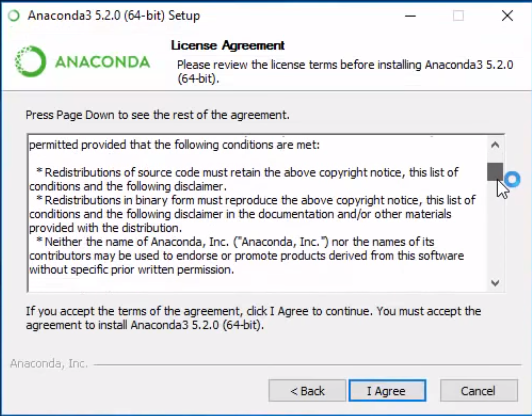
\includegraphics[width=6cm,height=6cm]{figures/gambar2.png}
\caption{Klik I Agree}
\label{akhir}
\end{figure}
\item Pilih sesuai yang anda inginkan tetapi saya merekomendasikan all user agar dapat dipakai oleh semua user
\begin{figure}[H]
\centering
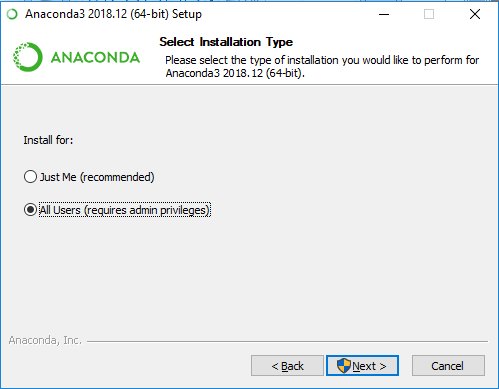
\includegraphics[width=6cm,height=6cm]{figures/gambar3.png}
\caption{Pilih sesuai yang anda inginkan}
\label{akhir}
\end{figure}
\item Pilih directory tempat anaconda akan diinstall lalu next
\begin{figure}[H]
\centering
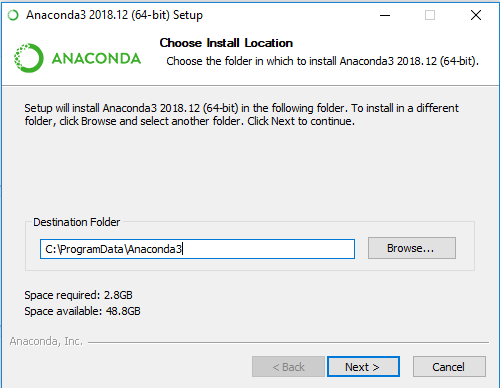
\includegraphics[width=6cm,height=6cm]{figures/gambar4.png}
\caption{Directory tempat anaconda akan diinstall}
\label{akhir}
\end{figure}
\item jika anda belum pernah menginstall python maka checklist keduanya dan jika anda sudah menginstall python maka checklist yang paling bawah saja
\begin{figure}[!htbp]
\centering
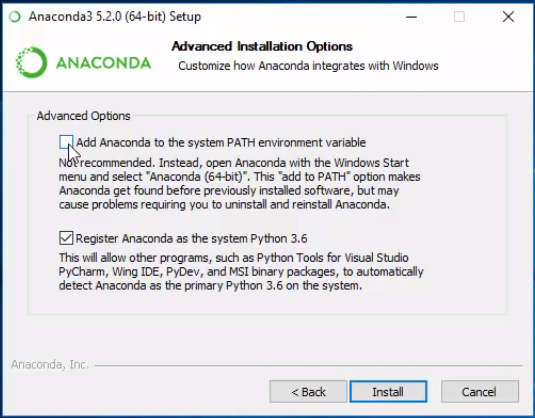
\includegraphics[width=6cm,height=6cm]{figures/gambar5.png}
\caption{Opsi Register}
\label{akhir}
\end{figure}
\item Tunggu hingga proses selesai lalu next
\begin{figure}[H]
\centering
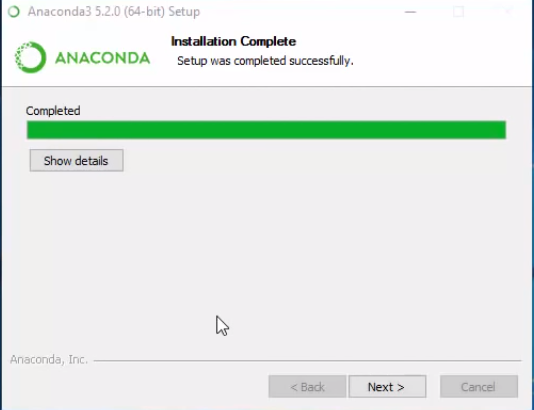
\includegraphics[width=6cm,height=6cm]{figures/gambar6.png}
\caption{Tunggu hingga selesai}
\label{akhir}
\end{figure}
\item Opsi tambahan untuk instal visual studio code, skip saja
\begin{figure}[H]
\centering
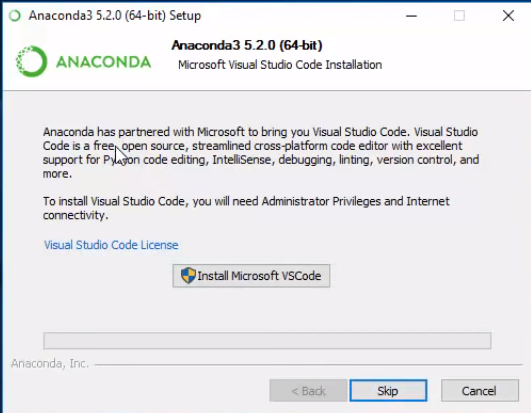
\includegraphics[width=6cm,height=6cm]{figures/gambar7.png}
\caption{Opsi Tambahan}
\label{akhir}
\end{figure}
\item uncheck semua dan click finish
\begin{figure}[H]
\centering
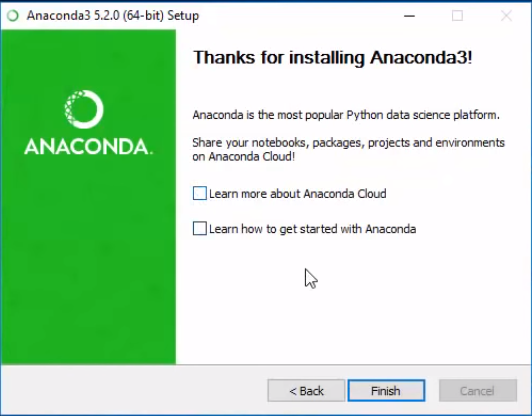
\includegraphics[width=6cm,height=6cm]{figures/gambar8.png}
\caption{Finish}
\label{akhir}
\end{figure}
\end{enumerate}

\subsection{Spyder}
\begin{enumerate}
\item Setelah install anaconda, buka aplikasinya.
\item Biasanya spyder sudah terinstall dengan anaconda, klik launch pada spyder
\begin{figure}[H]
\centering
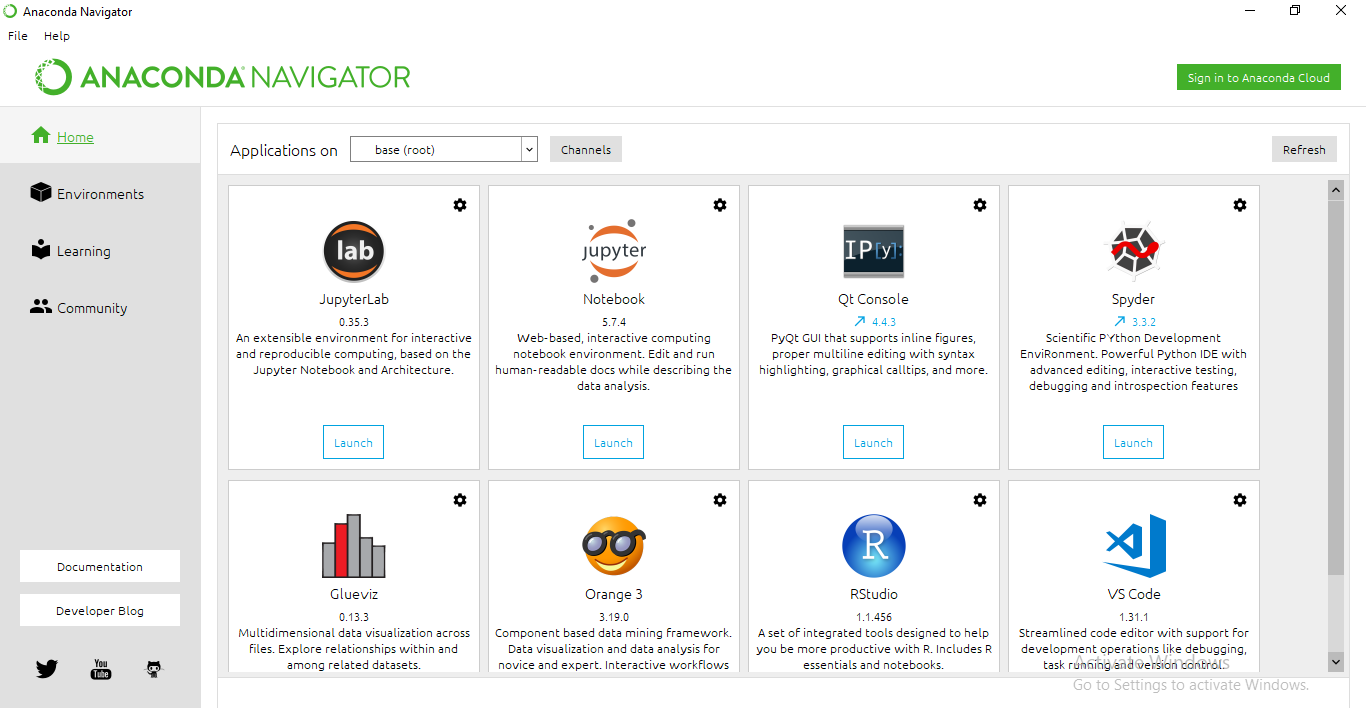
\includegraphics[width=6cm,height=6cm]{figures/gambar9.png}
\caption{Menu Utama Anaconda}
\label{Spyder}
\end{figure}
\item selesai, jika ingin melakukan percobaan maka ketik yang ada di bagian kiri lalu run atau F5
\begin{figure}[H]
\centering
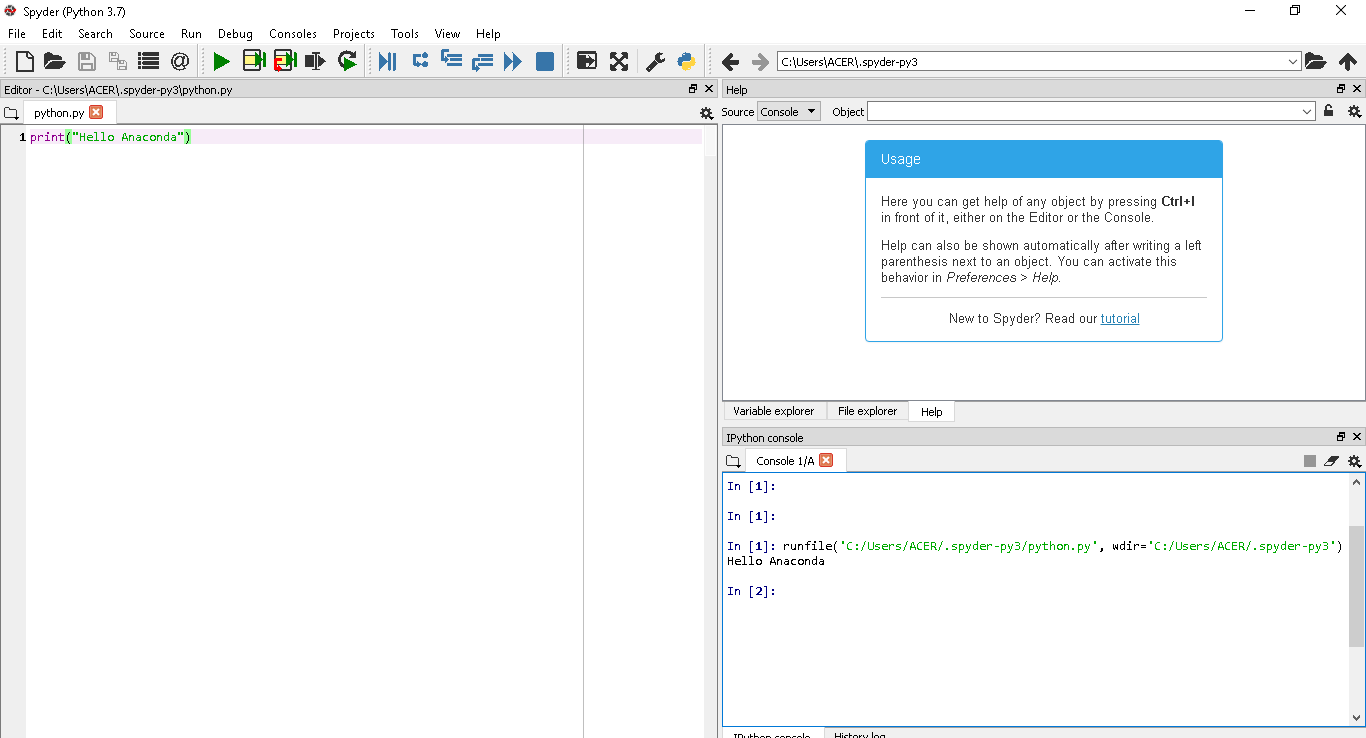
\includegraphics[width=6cm,height=6cm]{figures/10.png}
\caption{Spyder}
\label{akhir}
\end{figure}




\end{enumerate}
\section{Dini Permata Putri 1174053}
\subsection{Background}
Bahasa pemrograman saat ini jumlahnya sangat banyak. Python merupakan salah satu bahasa
pemrograman populer yang digunakan oleh banyak developer. Menurut survei bahasa pemrograman
versi www.tiobe.com, Python berada diperingkat ke-5 pada tahun 2016. Selain itu, Python juga bisa
digunakan untuk enterprise. Dalam tingkatan bahasa pemrograman, Python termasuk high level
language. Python menjadi salah satu bahasa pemrograman yang dapat digunakan untuk membangun
aplikasi, baik itu berbasis desktop, web ataupun berbasis mobile.



\begin{figure}[h!]
\centering
\includegraphics[scale=1.7]{universe}
\caption{The Universe}
\label{fig:universe}
\end{figure}

\documentclass[12pt]{Article}

\begin{document}  
\begin{center}
 Nama  : Nurul Izza Hamka \\
 Kelas : D4 TI 2C\\
 NPM   : 1174062
\end{center}
 
\section{Resume} 
\label{Resume}
\subsubsection{Resume Sejarah Python}

Python merupakan bahasa pemrograman yang bersifat interpretative. Python dikembangkan oleh Guido Van Rossum pada tahun 1990 di CWI, Amsterdam sebagai kelanjutan dari Bahasa pemrograman ABC. Nama Python dipilih oleh Guido sebagai nama bahasa ciptaanya karena kecintaannya pada televisi Monthy Python’s Flying Circus. Sekarang,distribusi python sudah mencapai versi 2.6.1 sampai dengan 3.0.\\

Pada tahun 1995 Guido pindah ke CNRI di Virginia Amerika sambil terus melanjutkan pengembangan Python. Versi terakhir yang dikeluarkan adalah 1.6. Tahun 2000, setelah itu Guido dan timnya berpindah lagi ke BeOpen.com dan dari sini mereka mengeluarkan Python versi 2.0.\\

Sampai sekarang pengembangan python terus dilakukan oleh pada pemrogram yang diambil alih oleh  Guido dan juga Python Softwa
re Foundation. 

\subsubsection{Perbedaan Python 2 dan 3}

Python versi 2 merupakan versi yang dikembangkan pada tahun 2000 dan yang paling banyak digunakan saat ini, baik dilingkungan produksi dan pengembangan, dan untuk membuka python 2 ini tinggal ketik python.\\
 
Sementara Python versi 3 adalah pengembangan lanjutan dari versi 2, yang terakhir rilis pada tahun 2008. Python 3 memiliki lebih banyak fitur dibandingkan Python 2, versi 3 ini ketika akan dibuka maka akan menggunakan perintah python3. Perubahan terbesar pada Python 3 termasuk memasukkan statemen print ke dalam built-in function.\\

Adapun perbedaan dari segi print:

Untuk Pyton 2 ketikkan menginput tidak menggunakan kurung biasa, namun pakek kurung juga bias dan dia menghasilkan atau mencetak satu baris. Sedangkan untuk python 3 harus menggunakan tanda kurung dan juga akan menghasilkan atau mencetak satu baris.\\

\subsubsection{Implementasi Python Di Perusahaan Dunia}

Ada beberapa perusahan terkenal dunia yang menggunakan bahasa Python, yaitu :\\
1. Google adalah perusahaan besar yang menggunakan banyak kode Python di dalam mesin pencarinya.\\
2. Youtube, situs video terbesar dan terpopuler di dunia, sebagian besar kodenya ditulis dalam bahasa Python.\\
3. Dropbox, menggunakan python baik di sisi server maupun di sisi pengguna layanannya.\\
4. ESRI, produsen terkenal pembuat software pemetaan GIS banyak menggunakan Python di produknya.\\
5. NASA, badan antariksa Amerika ini menggunakan Python untuk bidang sainsnya.
\section{Instalasi}
\subsubsection{Instalasi Python}

Cara Install Python di Windows\\
1. Unduh Python versi 3.7,\\
2. Buka file Python yang sudah di unduh,\\
3. Sebelum install pilih atau centang 'Add Python to PATH' di ujung kiri bawah
4. Pilih user, ada baiknya pilih 'Install For All Users' agak dapat di gunakan oleh semua user komputer,\\
5. Pilih Lokasi untuk menyimpan aplikasi Python,\\
6. Kemudian Next untuk melanjutkan,\\
7. Install untuk aplikasi Python Finish.
\subsubsection{Instalasi Anaconda}
Cara Install Python di Windows\\
1.Download aplikasi Anaconda di Windows, \\
2. Buka file Anaconda yang sudah di unduh,\\
3. Klik 'I Agree' pada perjanjian Lisensi,\\
4.Pilih user, ada baiknya pilih 'All Users' agak dapat di gunakan oleh semua user komputer,\\
5. Pilih Lokasi untuk menyimpan aplikasi Anaconda,\\
6. Ketika muncul dua pilihan, cukup centang 'Register Anaconda',\\
7.Install untuk Anaconda Complete.
\subsubsection{Script dan Intepreter Phyton}
Menggunakan Interpreter Python: \\
1. Jalankan interpreter. Buka Command Prompt, ketik python pada prompt dan tekan Enter. jika Python telah berhasil makan akan muncul tanda seperti ini (>>>).\\
2. Untuk menampilkan bantuan informasi kita dapat menggunakan perintah help()dan dapat dilakukan dengan 2 cara, yaitu dengan   help(int). Kedua adalah dengan mengetikan perintah help() didalam interpreter yang akan merubah mode interpreter ‘>>>’ menjadi mode ‘help>’.

\subsubsection{Pemakaian Spyder Variable explorer}
Explorer Variabel menunjukkan konten namespace, Variable Explorer Spyder menawarkan dukungan bawaan untuk mengedit daftar, string, dan kamus. Variable Explorer memiliki editor khusus, seperti :\\
- Integers\\
- Floats\\
- Complex numbers\\
- Strings
\section{Mencoba Python}
Membuat file lat1.py menggunakan teks Editor, kemudian ketikkan 'Hello Word!'. setelah itu simpan filelat1.py dan run menggunakan terminal.
\section{Identitas}
\subsubsection{Identitas dan Cara Menanganinya}
Excepetions berbeda dengan syntax error.Ketika tidak menangani exceptions dengan tepat, program-nya akan keluar secara paksa karena dia tidak tahu apa yang perlu dilakukan dalam kasus tersebut. Menangani banyak exception menggunakan satu klausa except dengan melwatkan exception tersebut ke klausa sebagai sebuah tuple.
\end{document}

\documentclass[lipt]{Article}
\begin{document}
\begin{center}
Aulyardha Anindita
D4 TI 2 C
1174054
\end{center}
\chapter{Resume}
\section{Sejarah Python}
Python adalah bahasa pemrograman yang mendukung multi paradigma pemrograman seperti pada pemrograman berorientasi objek, pemrograman imperatif, dan pemrograman fungsional. Python juga pada umumnya digunakan sebagai bahasa skrip walaupun pada praktiknya penggunaan python lebih luas. 

Bahasa pemrograman python dikembangkan oleh Guido van Rossum pada tahun 1990 di Stichting Mathematisch Centrum (CWI), Amsterdam yang merupakan kelanjutan dari bahasa pemrograman ABC dimana merupakan versi terakhir yang dikeluarkan oleh CWI adalah 1.2. Nama Python sendiri dipilih oleh Guido sebagai nama bahasa ciptaannya karena rasa cintanya pada acara televisi Monty Python’s Flying Circus.

Sekitar tahun 1995, Guido pindah ke CNRI di Virginia Amerika sambil dia melanjutkan pengembangan Python. Disinilah dia merilis beberapa versi dari python. Versi terakhir yang dikeluarkan saat itu adalah 1.6. Dan sekitar tahun 2000,  Guido dan timnya pindah ke BeOpen.com. BeOpen.com merupakan sebuah perusahaan komersial yang membentuk BeOpen PythonLabs. Python 2.0 dikeluarkan oleh BeOpen. Setelah mereka mengeluarkan Python 2.0, Guido dan beberapa anggota tim PythonLabs pindah ke DigitalCreations.
Dan pada tahun 2001, dibentuklah Organisasi Python yaitu Python Software  Foundation(PSF). PSF adalah suatu organisasi nirlaba yang dibuat untuk semua hal yang berkaitan dengan hak intelektual Python. 


\section{Perbedaan Python 2 dan Python 3}

Pada python 2 kita bisa menggunakan tanda kurung atau tidak sedangkan pada python3 kita wajib menggunakan tanda kurung, jika tidak maka kita akan mendapatkan hasil error.

Pada python 2 dalam melakukan sebuah inputan kita harus menggunakan “raw_input(‘teks’)”, sedangkan untuk python 3 kita hanya perlu menggunakan syntax “input(‘teks’)” saja.

Pada python2 dilengkapi dengan berbagai fitur programatikal seperti sysle-detecting garbage collector untuk mengotomasi manajemen memori, peningkatan dukungan untuk Unicode, list comprehension untuk membuat list berdasarkan dari list yang sudah ada. Sedangkan pada python 3 adalah melakukan perapian pada codebase dan menghapuskan duplikat atau redudansi.

\section{Implementasi dan Penggunaan Python di Perusahaan Dunia}
1.	Google adalah perusahaan besar yang menggunakan banyak kode Python di dalam mesin pencarinya. Dan mesin pencari google adalah yang paling terkenal di dunia.\\
2.	Youtube, situs video terbesar dan terpopuler di dunia, sebagian besar kodenya ditulis dalam bahasa Python.\\
3.	Facebook, media sosial terbesar di dunia, menggunakan Tornado, sebuah framework Python untuk menampilkan timeline.\\
4.	Instagram, siapa yang tidak kenal. Instagram menggunakan Django, framework python sebagai mesin pengolah sisi server dari aplikasinya.\\
5.	Pinterest, banyak menggunakan python untuk membangun aplikasinya.\\
6.	Dropbox, barangkali Anda adalah salah seorang pengguna layanan ini. Dropbox menggunakan python baik di sisi server maupun di sisi pengguna layanannya.\\
7.	Quora, salah satu situs tanya jawab terbesar di dunia, dibangun menggunakan Python.\\
8.	NASA, badan antariksa Amerika ini menggunakan Python untuk bidang sainsnya.\\
9.	NSA, badan mata – mata Amerika banyak menggunakan Python untuk analisa kriptografi dan intelijen.\\
10.	Industrial Light & Magic, Pixar, banyak menggunakan Python dalam animasi movie.\\
11.	Blender, Maya, software pembuat animasi 3D terkenal, menggunakan Python sebagai salah satu bahasa skrip pemrogramannya.\\
12.	Raspberry Pi, komputer mini yang banyak digunakan sebagai mikrokontroller, menggunakan Python sebagai bahasa utamanya.\\
13.	ESRI, produsen terkenal pembuat software pemetaan GIS banyak menggunakan Python di produknya.\\

\chapter{Instalasi}
\section{Proses Instalasi Python}
1. Download terlebih dahulu file Phyton nya. jika sudah didownload, maka kita masuk ke proses instalasi dengan mendouble klik pada file pyhton nya.\\
2. Centang Install launcher for all user untuk mengaktifkan python pada semua user Windows dan centang Python 3.6 to PATH untuk menambah path command Python. Kemudian klik Install Now. Klik Yes saat muncul notifikasi User Account Control. \\
3. Tunggu sampai proses instalasi selesai\\
4. Instalasi pyhton berhasil\\
5. Untuk mengetahui apakah pyhton nya sudah berjalan apa tidak yaitu dengan masuk ke Command Prompt dan ketikkan Phyton, jika ada berarti sudah tersambung\\

\section{Proses Instalasi Anaconda}
1. Download terlebih dahulu file Anaconda. Jika sudah didownload, maka langsung saja masuk ke proses instalasi dengan mendouble klik pada file Anacondanya.\\
2. Akan muncul tampilan pertama, lalu pilih next\\
3. Kemudian read lisensi dan klik I Agree\\
4. Kemudian pilih tempat penyimpanan nya, bagusnya yang default saja lalu pilih next\\
5. Kemudian pilih add anaconda to PATH atau tidak. Pilih apakah akan mendaftarkan Anaconda sebagai default Python 3.7?. Kecuali kita berencana menginstal dan menjalankan beberapa versi Anaconda, atau beberapa versi Python, biarkan default dan biarkan kotak ini dicentang. kemudian klik next.\\
6. Klik tombol Install. Jika Kita ingin melihat packages Anaconda yang sedang dipasang, klik Show Details, lalu pilih Next.\\
7. Untuk menginstal VS Code, klik tombol Install Microsoft VS Code. Setelah instalasi selesai, klik tombol Next Atau untuk menginstal Anaconda tanpa VS code, klik tombol skip. Memasang VS code dengan pemasang Anaconda membutuhkan koneksi internet. Pengguna offline mungkin dapat menemukan pemasang offline VS Code dari Microsoft.\\
8. Setelah proses instalasi berhasil, Kita akan melihat kotak dialog "Thanks for installing Anaconda3" lalu pilih Finish\\

\section{Cara Pemakaian Script dan Interpreter Python}
\subsection{Script}
1. Gunakan teks editor untuk menulis skrip\\
2. kemudian simpan dengan nama yang kalian inginkan\\
3. Kemudian untuk menjalankan skripnya, gunakan perintah berikut: python nama_skrip.py\\
4. Skrip python diterjemahkan ke dalam kode biner oleh (intepreter) python, sehingga komputer dapat mengerti arti perintah tersebut sehingga komputer mengerjakan perintah tersebut.\\
\subsection{Interpreter Python}
1. Membuka interpreter python pada submenu dari Aplikasi Python yang terdapat pada All Programs. Untuk keluar dari interpreter, ketik Ctrl+D / Ctrl+Q atau menggunakan perintah quit().\\
2. help() untuk menampilkan bantuan informasi kita dapat menggunakan perintah help(). Perintah help() dapat digunakan dengan 2 cara, yaitu dengan menggunakannya beserta object yang diinginkan, contohnya help(int). Kedua adalah dengan mengetikan perintah help() didalam interpreter yang akan merubah mode interpreter ‘>>>’ menjadi mode ‘help>’.\\
3. Setelah kita berada dalam mode ‘help>’ kita dapat langsung menggunakannya dengan memasukan keywords atau object yang diinginkan. Contohnya adalah keywords.\\
4. Jika kita mengetik salah satu keywords, maka interpreter akan memberikan informasi yang bersangkutan dengan keywords tersebut. Contohnya adalah if.\\
5. Disamping keywords kita juga dapat mendapatkan informasi tentang topics. Untuk mengetahui macam-macam topics, cukup dengan mengetikan perintah topics kedalam mode ‘help>’\\
6. Perintah topics memberikan informasi yang berguna kepada kita mengenai bahasa pemrograman python. Selain cara help() diatas, kita juga dapat menggunakan cara yang kedua yaitu langsung bersama object yang diinginkan misalnya adalah string. Untuk mencobanya ketik help(str)\\
7. Dengan menggunakan perintah help(str) kita dapat mengexplore object string beserta attribut dan method-method yang dimilikinya. Dan hal tersebut berlaku untuk semua keywords python. Tanda titik dua diatas menandakan informasi yang disampaikan masih bersambung, untuk mengetahui informasi selanjutnya tekan space sampai muncul kata (END)\\

\section{Cara Pemakaian Spyder Termasuk Variable Explorer}
1. Variable Explorer Spyder menawarkan dukungan bawaan untuk mengedit daftar, string, kamus, array NumPy, Pandas DataFrames, dan banyak lagi, dan dapat juga histogram, plot, atau bahkan menampilkan beberapa di antaranya sebagai gambar RGB.\\
2. Variable Explorer memiliki editor khusus untuk serangkaian objek Python internal dan pihak ketiga yang umum, dan dapat melihat, mengedit, dan mengintrospeksi objek paling arbitrer secara mendalam melalui Penjelajah Objek yang lebih umum\\

\chapter{Mencoba Phyton}
print ("Hello World Python!")

\chapter{Identasi}
Indentasi merupakan keluarnya suatu teks/naskah dari batas kiri, batas kanan atau keduanya. Kita dapat mengatur indentasi hanya pada baris pertama (first line indent) dari paragraf atau mengatur indentasi mengandung (hanging).\\

Cara mengatasinya yaitu dengan mensetting ulang indent nya, mengatur panjang indent. sehingga ruas kiri dan kanan nya menjadi rata.



\end{document}

\documentclass{article}
\usepackage[utf8]{inputenc}
\begin{document}
Ilham Muhammad Ariq 
\par
D4TI2C
\par
1174087
\section{Mengenal Python dan Anaconda}
\begin{enumerate}
    \item 
{SEJARAH PYTHON}
\par
{Pyhton dikembangkan pada tahun 1990 oleh Guido van Rossum di CWI Amsterdam sebagai kelanjutan dari bahasa pemrograman ABC.}
\par
{Tahun 1995, Guido pindah ke CNRI di Virginia Amerika sambil terus melanjutkan pengembangan Python. Versi terakhir yang dikeluarkan adalah 1.6. Tahun 2000, Guido dan para pengembang inti Python pindah ke BeOpen.com yang merupakan sebuah perusahaan komersial dan membentuk BeOpen PythonLabs. Python 2.0 dikeluarkan oleh BeOpen. Setelah mengeluarkan Python 2.0, Guido dan beberapa anggota tim PythonLabs pindah ke DigitalCreations.
\par
Saat ini pengembangan Python terus dilakukan oleh sekumpulan pemrogram yang dikoordinir Guido dan Python Software Foundation. Python Software Foundation adalah sebuah organisasi non-profit yang dibentuk sebagai pemegang hak cipta intelektual Python sejak versi 2.1 dan dengan demikian mencegah Python dimiliki oleh perusahaan komersial. Saat ini distribusi Python sudah mencapai versi 2.7.14 dan versi 3.6.3
\par
Nama Python dipilih oleh Guido sebagai nama bahasa ciptaannya karena kecintaan Guido pada acara televisi Monty Python's Flying Circus. 
    \item
PERBEDAAN PYTHON 2 DAN 3
\par
Python versi 2 merupakan versi yang banyak digunakan saat ini, baik dilingkungan produksi dan pengembangan.Sementara Python versi 3 adalah pengembangan lanjutan dari versi 2. Python 3 memiliki lebih banyak fitur dibandingkan Python 2. Untuk membuka Python 2 kita hanya menggunakan perintah python saja, sedangkan Python 3 menggunakan perintah python3.
 }   
\end{enumerate}

\section{Background}
Bahasa pemrograman saat ini jumlahnya sangat banyak. Python merupakan salah satu dari bahasa pemrograman populer yang digunakan oleh banyak developer. Dalam tingkat bahasa pemrograman, Python termaksud high level language. Python menjadi salah satu bahasa pemrograman yang dapat digunakan untuk membangun aplikasi, baik itu berbasis desktop, web atau berbasis mobile. 
Python memiliki beberapa web framework salah satunya django. Django merupakan sebuah web framework berbasis Python yang mendukung perbuatan sebuah website secara rapid development dengan desain yang elegan. Django merupakan web framework yang dirancang dan dibangun oleh Andrian Holovaty dan Jacob Kaplan Moss. Menurut survei framework python versi  hotframeworks.com, framework Django berada diperingkat pertama.



\section{Problems}

1. Bagaimana cara mengembangkan bahasa pemrograman python?

2. Apakah peranan python sangat dibutuhkan sekarang?

3. Apa-apa saja framework yang terdapat dari python \citep{adams1995hitchhiker}



\section{Objective and Contribution}


\section{Objective}
Objectif dalam bahasa pemrograman python adalah agar mahasiswa D4 Teknik Informatika bisa memahami materi python dan bisa mengembangkan pengetahuannya mahasiswa.




\section{Contribution}
kontribusi adalah peran dimana peran python sangatlah baik digunakan mahasiswa karena python adalah bahasa pemrograman yang sangat efektif dan efisien.



\section{scoop and environtment}

1.Topik dan pembelajaran dengan bahasa python 

2.Pengaruh peranan bahasa pemrograman pytho

3.framework-framework python yang mudah digunakan
\bibliographystyle{}
\bibliography{}
\section{Cara Pemakaian Python}
\par
Untuk menuliskan script Python, cukup buka terminal yang ingin digunakan misalkan cmd dan ketikan pyhton
contoh syntax dasar Hello word
\par
ketikan :
\par
print('hello word')
\par
outputnya :
\par
hello word

\section{Instalasi Python}
\begin{enumerate}
\item
Download file python terlebih dahulu
\item
Kemudian install file yg telah didownload
\item
Pilih saja ‘Install for all users’ agar bisa dipakai untuk semua user di komputernya
\item
Tentukan lokasi python akan diinstal, kemudian klik next.
\item
Pada tahapan ini, kita akan menentukan fitur-fitur yang akan diinstal.
Jangan lupa untuk mengaktifkan ‘Add python.exe to path’ agar perintah python dikenali pada CMD (Command Prompt).
\end{enumerate}

\section{Indentasi}
\par
Python memanfaatkan indentasi untuk membuka/menutup fungsi tersebut. jika melakukan coding dengan notepad++. Pada notepad++ setting perintah Tab menjadi indentasi 4 karakter spasi , dengan memilih Setting -> Preferences ceklist box Replace by Space dengan Tab Size = 4.Dengan begitu yang tinggal mengklik ‘Tab‘ pada keyboard untuk melakukan indentasi kedalam, tanpa harus  mengisi dengan spasi sebanyak 4 kali.
\end{document}

\begin{document}

\section{Resume}
\begin{flushleft}
\qquad Python dibuat oleh Guido van Rossum yang dirilis pertama  kali pada tahun 1992, 'python 1.0' dirilis pada januari 1994 dan versi terakhir yang ini dirilis saat ini adalah 'Python 3.7' pada 27 Juni 2018. Nama Python sendiri diambil dari acara televisi Monty Python's Flying Circus. Python mendukung multi paradigma pemrograman. pengembangan Python masih dilakukan oleh Team Guido dan Python Software Foundation sebagai pemegang hak cipta intelektual Python sejak versi 2.1 . perbedaan antara python2 dan python3 contohnya pada statement print, pada python2 : 

print "Hello World"

sedangkan pada python3 :

print ("Hello World")
\end{flushleft}

\section{Instalasi}
\subsection{Install Anacaconda}
\begin{enumerate}
\item Download Anaconda3 https://www.anaconda.com/distribution/#linux
\item 'bash Anaconda3-2018.12-Linux-x86-64.sh
\item review license agreement
\item agree license agreement, text 'yes'
\item lokasi install default di /root/anaconda3
\item tambahkan lokasi di /root/.bashrc, text 'yes'
\item selesai
\end{enumerate}

\subsection{Install Python}
\begin{enumerate}
\item apt-get install python3
\item selesai
\end{enumerate}

\subsection{Install Python pip}
\begin{enumerate}
\item apt-get install python3-pip
\item selesai
\end{enumerate}


\end{document}


\section{MuhammadRezaSyachrani/1174084}
\subsection{Background}
	Python merupakan salah satu bahasa pemrograman tingkat tinggi (high level language) yang dikembangkan oleh Guido van Rossum pada tahun 1989 dan diperkenalkan untuk pertama kalinya pada tahun 1991 di Scitchting Mathematisch Centrum (CWI).
	Python dirancang untuk memberikan kemudahan bagi programmer melalui segi efisiensi waktu, kemudahan dalam pengembangan dan kompatibilitas dengan sistem. Python bisa digunakan untuk membuat aplikasi standalone (berdiri sendiri) dan
	pemrograman script (scripting programming).
	\par
	Python adalah bahasa pemrograman interpretatif multiguna dengan filosofi perancangan yang berfokus pada tingkat keterbacaan kode. Python diklaim sebagai bahasa yang menggabungkan kapabilitas, kemampuan, dengan sintaksis kode yang sangat jelas,
	dan dilengkapi dengan fungsionalitas pustaka standar yang besar serta komprehensif. 
	Sisi utama yang membedakan Python dengan bahasa pemrograman lain adalah dalam hal aturan penulisan kode
	program. Programmer yang menggunakn selain python dapat dibingungkan dengan aturan indentasi, tipe data,
	tuple, dan dictionary. Python memiliki kelebihan tersendiri dibandingkan dengan bahasa lain terutama
	dalam hal penanganan modul, ini yang membuat beberapa programmer menyukai python. Selain itu
	python merupakan salah satu produk yang opensource, free, dan multiplatform.
	
\subsection{Problems}
\begin{itemize}
	\item Bagaimana cara mengimplementasikan bahasa pemrograman python
\end{itemize}
	
\subsection{Objective and Contribution}
\subsubsection{Objective}
\begin{itemize}
	\item Dapat mengimplementasikan bahasa pemrograman python
\end{itemize}
	
\subsubsection{Contribution}
\begin{itemize}
	\item Dapat membangun suatu aplikasi dan alat yang mengimplementasikan bahasa pemrograman python
\end{itemize}


\subsection{Scoop and Environtment}
\begin{itemize}
	\item Menginplementasikan Python dalam pemrograman
\end{itemize}


\subsection{Problems}
1. bagaimana proses belajar bahasa pemrograman phyton?
2. bagaimana cara cepat menguasai bahasa pemrograman phyton?

\subsection{Objective and Contribution}
Mahasiswa D4 Teknik Informatika mempelajari dan memahami Bahasa Pemrograman Phyton.

\subsection{Scoop and Environment}
1. belajar bahasa pemrograman phyton sangat efektif
2. cukup mudah untuk memahami bahasa pemrograman phyton


\bibliographystyle{}
\bibliography{}
\section{Identasi}
Ketika menulis kode program Python perlu memperhatikan indentasi, karena kode program Python distrukturkan berdasarkan indentasi. Kode program yang berada pada sisi kiri yang sama maka dibaca sebagai satu blok, untuk membuat sub blok maka cukup dengan memberikan jarak spasi atau tab ke kanan.
Soal indentasi ini akan lebih jelas ketika pembahasan tentang pencabangan, perulangan, fungsi, class, dan materi yang lain yang membutuhkan penulisan kode program bersarang.
Contohnya adalah sebagai berikut:
import sys
\paragraph{}
if len(sys.argv) < 2:
\paragraph{}
    print("Harap memasukkan argumen.")
    \paragraph{}
    sys.exit(1)

	\section{AlvanAlvanzah/1174077}
\subsection{Background}
Python adalah bahasa pemrograman interpretatif multiguna dengan filosofi perancangan yang berfokus pada tingkat keterbacaan kode. Python diklaim dijadikan bahasa yang menggabungkan kapabilitas, kesanggupan, dengan sintaksis kode yang sangat jelas, dan dilengkapi dengan fungsionalitas pustaka standar yang besar serta komprehensif.
\par
Python adalah bahasa pemrograman yang bersifat open source. Bahasa pemrograman ini dioptimalisasikan untuk software quality, developer productivity, program portability, dan component integration. Python telah digunakan untuk mengembangkan berbagai macam perangkat lunak, seperti internet scripting, systems programming, user interfaces, product customization, numberic programming dll. Python saat ini telah menduduki posisi 4 atau 5 bahasa pemrograman paling sering digunakan di seluruh dunia. Menggunakan alat pihak ketiga, kode Python dapat dikemas ke dalam program yang dapat dieksekusi mandiri. Penerjemah python tersedia untuk banyak sistem operasi.
\subsection{Problems}
\begin{itemize}
\item Bagaimana cara agar memahami bahasa pemrograman python
\end{itemize}
\subsection{Objective and Contribution}
\subsubsection{Objective}
\begin{itemize}
\item Dapat memahami bahasa pemrograman Python
\end{itemize}
\subsubsection{Contribution}
\begin{itemize}
\item Dapat mengimplementasikan bahasa pemrograman python
\end{itemize}

\subsection{Scoop and Environtment}
\begin{itemize}
\item Mempelajari tentang bahasa pemrograman python
\end{itemize}

